\chapter{Apresentação Teórica}
\label{ch:02-background}

We can make human language manageable to computers by using a sort of different methods and techniques. This is the bread and butter of any NLP researcher. Here, following the NLP community, we will focus only in the techniques derived from the machine learning field. In this chapter, we will present some abstract machine learning models follow by some applications in NLP. 

\section{Redes Neurais}

Uma rede neural é, essencialmente, um modelo de aprendizado de máquina supervisionado %[ref] 
que está a procura de aprender \textit{padrões}. A inspiração para o desenvolvimento desse tipo de modelagem surgiu a partir de estudos em neurosciência %[ref] 
que concluiram que, diante de múltiplas apresentações de um mesmo estímulo, um mesmo grupo de neurônios sofre incitação e dispara%[ref david hubel ]
.  Analogamente, o modelo artificial é composto por uma camada de \textit{input} (um vetor) que recebe diferentes estímulos (\textit{features}). A informação recebida é processada e distribuída ao longo de múltiplas conexões com a próxima camada. Tais conexões são representadas por uma matriz \textbf{W} de pesos que passa por uma função de ativação\footnote{Diferentes funções de ativação podem ser utilizadas, como por exemplo a Softmax, a RELU, a Tanh ou a própria Sigmoid apresentada no texto.}. A função de ativação aqui, funciona como uma forma de administração dos disparos dos neurônios, de modo a condicionar a probabilidade de disparo à equação \ref{eq:sigmoid}. Também é uma maneira de garantir ao sistema a produção de diferentes respostas para padrões diferentes utilizando a mesma rede. Além disso, permite com que o aprendizado ocorra de forma gradual, de modo que o efeito de estímulos passados ainda perdure por um longo período mesmo após a apresentação de novos estímulos 
\begin{figure}[h]
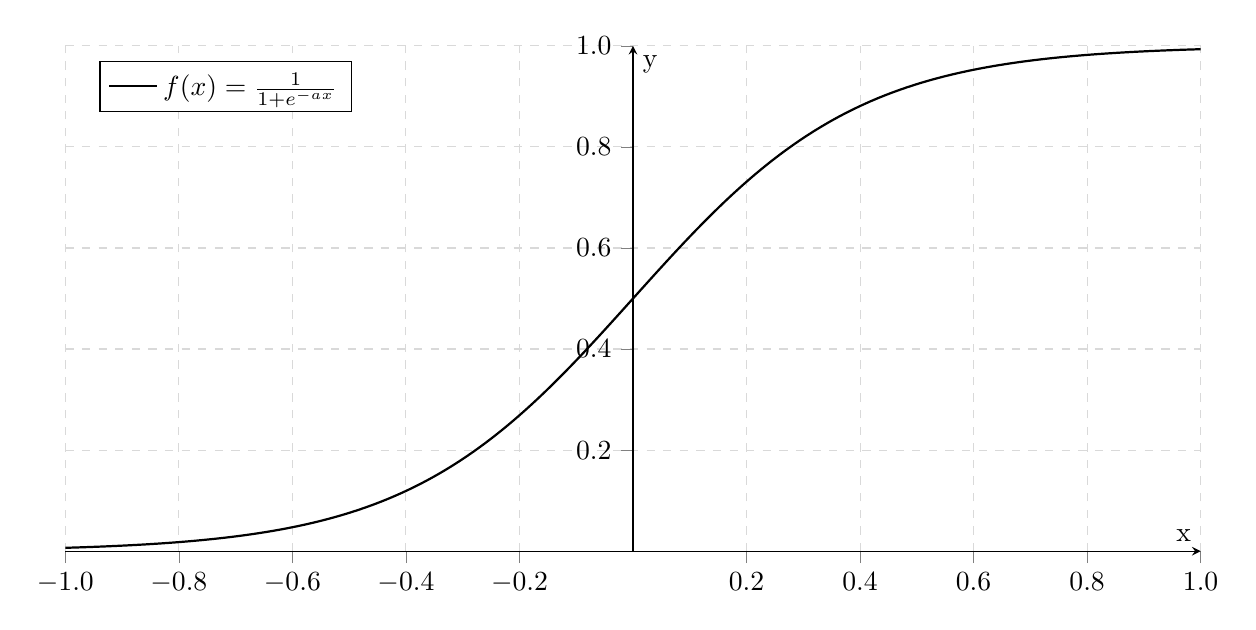
\begin{tikzpicture}
    \begin{axis}[
    	legend pos=north west,
        axis x line=middle,
        axis y line=middle,
        x tick label style={/pgf/number format/fixed,
                            /pgf/number format/fixed zerofill,
                            /pgf/number format/precision=1},
        y tick label style={/pgf/number format/fixed,
                            /pgf/number format/fixed zerofill,
                            /pgf/number format/precision=1},
        grid = major,
        width=16cm,
        height=8cm,
        grid style={dashed, gray!30},
        xmin=-1,     % start the diagram at this x-coordinate
        xmax= 1,    % end   the diagram at this x-coordinate
        ymin= 0,     % start the diagram at this y-coordinate
        ymax= 1,   % end   the diagram at this y-coordinate
        %axis background/.style={fill=white},
        xlabel=x,
        ylabel=y,
        tick align=outside,
        enlargelimits=false]
      % plot the stirling-formulae
      \addplot[domain=-1:1, black, thick,samples=500] {1/(1+exp(-5*x))};
      %\addplot[domain=-1:1, blue, ultra thick,samples=500] {1/(1+exp(-10*x))};
      \addlegendentry{$f(x)=\frac{1}{1+e^{-ax}}$}
      %\addlegendentry{$g(x)=\frac{1}{1+e^{-10x}}$}
    \end{axis} 
\end{tikzpicture}
\caption{A função logística utilizada para o cálculo da probabilidade de ativação.}
\label{fig:sigmoidplot}
\end{figure}
(Fig. \ref{fig:sigmoidplot}). Após essa transformação, o resultado serve como novo input para a próxima camada e assim sucessivamente até a última, a camada de \textit{output}.

\begin{align}\label{eq:sigmoid}
p(w_{i} = 1) = \frac{1}{1+e^{\sum_{i} w_{i}x_{i} + b}}
\end{align}

Algebricamente, pode-se representar o processo descrito através da composição de múltiplas funções, uma vez que o resultado das operações precedentes servirão como entrada para as próximas camadas.

\begin{align}
f(\vect{x}; \vect{\theta}) &= f^{(2)}(f^{(1)}(\vect{x}; \vect{W}_1, \vect{b}_1); \vect{W}_2, \vect{b}_2)\\
&= \sigma(\vect{W}_2 (\sigma(\vect{W}_1\vect{x} + \vect{b}_1)) + \vect{b}_2)
\end{align}

\subsection{Treinamento}

Para que a rede seja capaz de identificar os padrões desejados, é necessário alimentá-la com o que se espera como resposta (\textit{targets}), pois o treinamento da mesma consiste, essencialmente, na atualização das matrizes de pesos que deve ocorrer a partir da comparação entre os valores previstos pela rede (\textit{outputs}) e os \textit{targets}. A comparação entre esses valores se dá por meio de uma função de custo (\textit{Loss Function}), que representa uma forma de se quantificar o quão perto se está de uma rede ideal em que os outputs correspondam exatamente aos targets. Nesse sentido, encontrar o mínimo desta função significa também encontrar os melhores pesos para o aprendizado da tarefa em questão.
%colocar a referencia do Deep Learning, a practioneers approach

\section{Modelagem em Redes Neurais para os Verbos do Português Brasileiro}

O esquema apresentado pelos pesquisadores Rumelhart e McClelland represetado na Fig. \ref{fig:esquemafdd} é conhecido como uma arquitetura do tipo \textit{Feed-Forward-Network (FFD)} porém sem camadas intermediárias. Nesse caso, todos os nódulos da camada de input se conectam diretamente aos nódulos da camada de output.

Por se tratarem de dados linguísticos (caracteres), os pesquisadores apresentam a codificação dos fonemas em representações vetoriais, introduzindo portanto a noção de \textit{Wickelfeatures}.

\subsection{Wickelfeatures}
\label{sec:wickelfeatures}
Como descrito na Seção \ref{ch:01-introduction}, as unidades de input e output correspondem às features fonéticas que caracterizam os verbos no tempo presente. Rumelhart e McClelland propõe a caracterização de cada fonema como uma combinação de features em apenas 4 dimensões. O fonema \textit{d}, por exemplo, é caracterizado por um conjunto de 4 features: Consoante Interrompida, Vozeada, - e -. %Stop ? e Middle?.
Nesse sentido, os pesquisadores apresentam uma tabela que codifica cada fonema na língua inglesa às quatro dimensões de features. A Tabela \ref{tab:Tab1} foi baseada nesse sistema de codificação, porém simplificado e adaptado para o português brasileiro. A primeira dimensão da tabela divide os fonemas em três grandes grupos: consoantes interrompidas, continuadas ou vogais. A segunda dimensão aumenta o grau de resolução da primeira e ainda as divide em stops e nasais, %ver traducoes
fricativas e líquidas, altas e baixas. A terceira dimensão classifica os fonemas de acordo com três simples pontos de articulação: Frontal, Média ou Back. %ver traducao para Back.
A quarta dimensão subcategoriza as consoantes em vozeadas vs. não-vozeadas e as vogais em longas e curtas. A presença de cada uma destas features em um determinado fonema recebe o valor $1$, enquanto que a ausência, $0$.
Com base na tabela %ref
portanto, o fonema \textit{d} passa a ser representado pelo vetor:

\begin{align}
d \Rightarrow (100)(10)(010)(10)
\end{align}

Contudo, por se tratarem de dados linguísticos, é imprescindível que a própria sequência fonológica também seja representada. Desse modo, os pesquisadores optam por representar, em cada vetor de input, uma sequência de três features (uma feature para cada fonema subsequente) para cada uma das dimensões propostas. Por fim, é feita uma última ressalva. Após o treinamento da rede, é necessária a criação de uma função capaz de decodificar os resultados obtidos pela camada de output. O problema se dá pois, uma vez que os vetores são introduzidos na rede, a noção de sequência se perde. Para solucionar este problema, os pesquisadores introduzem mais uma última dimensão a cada fonema, a dimensão de \textit{boundary}. Com isso, o \textit{token} de '\#' é introduzido ao início e ao fim de cada um dos verbos para "notificar" à rede de que ela está processando um item de início ou final de palavra. Desse modo, as equações \ref{token1} e \ref{token2} exibem as representações vetoriais do token de boundary e dos fonemas \textit{d} e \textit{a} considerando a última dimensão mencionada.

\begin{align}
\# \Rightarrow (000)(00)(000)(00)(1)\label{token1}\\
d \Rightarrow (100)(10)(010)(10)(0)\label{token2}\\
a \Rightarrow (001)(01)(010)(01)(0)\label{token3}
\end{align}

Por fim, cada dimensão de um fonema pode ser combinado com todas as dimensões do próximo fonema da sequência, ou seja, procura-se estudar não somente a relação entre as consoantes interrompidas e as vogais, mas também entre as consoantes interrompidas e formações fonéticas com ponto de articulação médio. Os pesquisadores definem como um \textit{Wickelfeature} cada sequência de três features fonéticas e é esta informação que serve como entrada para a rede neural responsável por detectar as irregularidades verbais.


\begin{table}[ht!]
\center
    \begin{tabular}{lrrrrrrr}\toprule
        &\multicolumn{2}{c}
{}&\multicolumn{1}{c}     {\textbf{Anterior}}&\multicolumn{2}{c}{\textbf{Médio}}&\multicolumn{2}{c}{\textbf{Posterior}}
        \\\cmidrule(r){3-4}\cmidrule(r){5-6}\cmidrule(r){7-8}   
        &&V/L&U/S&V/L&U/S&V/L&U/S\\\midrule
        Int.&    Stop & b & p
                & d & t
                & g & k\\
                &Nasal & m
                & & n
                & & 
                & \\
        Cont. & Fricat. & v& f
                & z & s
                & j & x\\
                &Liq. &l
                & &r
                & &
                & h\\
        Vowel & Alta & e & i 
                &   &  
                & o & u\\
              & Baixa & & E
              & &a
              & & O
        \\\bottomrule
    \end{tabular}
    \caption{Categorização de fonemas em quatro dimensões adaptada ao Português Brasileiro}\label{tab:Tab1}
\end{table} 

\subsection{Codificação}
\label{sec:cod}
Cada verbo que participa da etapa de treinamento da rede passa por um processo inicial de codificação. Tal processo é descrito a seguir utilizando o verbo \textit{dar} como exemplo.\\ 

\textbf{Entrada:} \textit{dar}\\

\textbf{Passo 1:} O token de início e final de palavra é acrescentado:\\
\hspace*{6.0em}      \#dar\#\\

\textbf{Passo 2:} O verbo é segmentado em trigramas:\\
\hspace*{6.0em}\#,d,a - d,a,r - a,r,\#\\

\textbf{Passo 3:} Um dicionário associa cada fonema a um vetor de features fonéticas.\\

\textbf{Passo 4:} As features dos trigramas são combinadas produzindo \textit{Wickelfeatures}.\\

%alterar a identacao aqui
Exemplos:
\begin{itemize}
\item boundary - int - vowel 
\item boundary - stop - low
\item boundary - middle - middle
\item middle - middle - liq
\item stop - low - cont
\item ...
\end{itemize}


\textbf{Passo 5:} Um vetor-dicionário de dimensão correspondente ao número total de combinações de features possíveis é inicializado com $0's$ em todas as casas.\\

\textbf{Passo 6:} Cada combinação de features existente no verbo analisado altera o valor do vetor-dicionário para $1$.\\

\textbf{Passo 7:} O vetor-dicionário atualizado é utilizado como \textit{input} para a rede.

\subsection{Decodificação}
\label{sec:dec}

%falar brevemente sobre a dificuldade de se decodificar esses valores

\section{Redes Neurais Recorrentes}
\label{sec:RNN}

A Seção \ref{sec:wickelfeatures} serve de exemplo para evidenciar a dificuldade ao se utilizar a arquitetura FFN na modelagem de dados sequencias. Certamente, os processos descritos nas subseções \ref{sec:cod} e \ref{sec:dec} não se apresentam como componentes simples ou orgânicos, tão pouco eficientes. O problema anunciado pela modelagem desse tipo de dado motivou o desenvolvimento de uma nova família de redes neurais, as Redes Neurais Recorrentes (\textit{Recurrent Neural Network - RNN}). 

A ideia central desse modelo consiste na retroalimentação dos elementos sequenciais, de modo que o \textit{input} de cada um deles serve, não somente para a previsão do próximo item da sequência, mas também para a formação de um componente intermediário, um \textit{estado}. Esses estados, representados na Figura \ref{fig:unfoldedrnn} como $\vect{h}$'s %colocar notacao de vetor aqui
funcionam como uma espécie de memória condensada dos elementos precedentes e influenciam diretamente os estados posteriores. Essa é uma maneira de retransmitir a cada momento os efeitos dos inputs anteriores para o restante da sequência.

%\definecolor{blue}{RGB}{159, 192, 176}
\definecolor{green}{RGB}{160, 227, 127}
\definecolor{orange}{RGB}{243, 188, 125}
\definecolor{red}{RGB}{253, 123, 84}
\definecolor{nephritis}{RGB}{39, 174, 96}
\definecolor{emerald}{RGB}{46, 204, 113}
\definecolor{turquoise}{RGB}{39, 174, 96}
\definecolor{green-sea}{RGB}{22, 160, 133}
\definecolor{purple}{RGB}{181, 124, 215}
% Tikzstyles for Computation Graphs

% nodes
\tikzstyle{noop} = [circle, draw=none, fill=red, minimum size = 10pt]
\tikzstyle{op} = [circle, draw=red, line width=1.5pt, fill=red!70, text=black, text centered, font=\bf \normalsize, minimum size = 25pt]

\tikzstyle{opintense} = [circle, draw=red, line width=1.5pt, fill=red!150, text=black, text centered, font=\bf \normalsize, minimum size = 25pt]


%new style
\tikzstyle{gp} = [circle, draw=red, line width=4pt, text=black, text centered, font=\bf \normalsize, minimum size = 4.cm]

\tikzstyle{box} = [rectangle, draw=red, line width=1.5pt, fill=red!70, text=black, align=center, font=\bf \normalsize, minimum size = 45pt]

\tikzstyle{state} = [circle, draw=blue, line width=1.5pt, fill=blue!70, text=black, text centered, font=\bf \normalsize, minimum size = 25pt]

\tikzstyle{output} = [circle, draw=purple, line width=1.5pt, fill=purple!70, text=black, text centered, font=\bf \normalsize, minimum size = 25pt]


\tikzstyle{gradient} = [circle, draw=nephritis, line width=1.5pt, fill=nephritis!60, text=black, text centered, font=\bf \normalsize, minimum size = 25pt]
\tikzstyle{textonly} = [draw=none, fill=none, text centered, font=\bf \normalsize]
\tikzstyle{boxtextonly} = [draw=none, fill=none, align=center, font=\bf \normalsize]

\tikzstyle{normal} = [circle, draw=black, line width=1.0pt, fill=none, text=black, text centered, font=\bf \normalsize, minimum size = 20pt]


% edges
\tikzstyle{tedge}  = [draw, thick, >=latex, ->]
\tikzstyle{tedge_dashed}  = [draw, thick, >=latex, ->, dashed]
\tikzstyle{nedge}  = [draw, thick, >=latex]
\tikzstyle{nedge_dashed}  = [draw, thick, >=latex, dashed]


% namedscope
\tikzstyle{namedscope} = [circle, draw=orange, line width=1.5pt, fill=orange!60, align=center, inner sep=0pt]
\begin{figure}[ht!]
\centering

\scalebox{1.40}{
\begin{tikzpicture}[auto]

% RNN state cell =============================
\node[normal] (h) {$\vect{h}$};
\node[normal, below=30pt of h] (x) {$\vect{x}$};
\node[normal, above=30pt of h] (yhat) {$\hat{\vect{y}}$};



% edges
\path[tedge] (x) edge node[below right= -4pt] {}  (h) ;
\path[tedge] (h) edge [out=-400,in=-320,looseness=8, distance=125pt] node[above right] {} (h);
\path[tedge] (h) edge node[below right = -4pt] {} (yhat);


\end{tikzpicture}

} % scalebox
\caption{Representação Simplificada de uma RNN}
\label{fig:RNN1}
\end{figure}
\definecolor{blue}{RGB}{159, 192, 176}
\definecolor{green}{RGB}{160, 227, 127}
\definecolor{orange}{RGB}{243, 188, 125}
\definecolor{red}{RGB}{253, 123, 84}
\definecolor{nephritis}{RGB}{39, 174, 96}
\definecolor{emerald}{RGB}{46, 204, 113}
\definecolor{turquoise}{RGB}{39, 174, 96}
\definecolor{green-sea}{RGB}{22, 160, 133}
\definecolor{purple}{RGB}{181, 124, 215}
% Tikzstyles for Computation Graphs

% nodes
\tikzstyle{noop} = [circle, draw=none, fill=red, minimum size = 10pt]
\tikzstyle{op} = [circle, draw=red, line width=1.5pt, fill=red!70, text=black, text centered, font=\bf \normalsize, minimum size = 25pt]

\tikzstyle{opintense} = [circle, draw=red, line width=1.5pt, fill=red!150, text=black, text centered, font=\bf \normalsize, minimum size = 25pt]


%new style
\tikzstyle{gp} = [circle, draw=red, line width=4pt, text=black, text centered, font=\bf \normalsize, minimum size = 4.cm]

\tikzstyle{box} = [rectangle, draw=red, line width=1.5pt, fill=red!70, text=black, align=center, font=\bf \normalsize, minimum size = 45pt]

\tikzstyle{state} = [circle, draw=blue, line width=1.5pt, fill=blue!70, text=black, text centered, font=\bf \normalsize, minimum size = 25pt]

\tikzstyle{output} = [circle, draw=purple, line width=1.5pt, fill=purple!70, text=black, text centered, font=\bf \normalsize, minimum size = 25pt]


\tikzstyle{gradient} = [circle, draw=nephritis, line width=1.5pt, fill=nephritis!60, text=black, text centered, font=\bf \normalsize, minimum size = 25pt]
\tikzstyle{textonly} = [draw=none, fill=none, text centered, font=\bf \normalsize]
\tikzstyle{boxtextonly} = [draw=none, fill=none, align=center, font=\bf \normalsize]

\tikzstyle{normal} = [circle, draw=black, line width=1.0pt, fill=none, text=black, text centered, font=\bf \normalsize, minimum size = 20pt]


% edges
\tikzstyle{tedge}  = [draw, thick, >=latex, ->]
\tikzstyle{tedge_dashed}  = [draw, thick, >=latex, ->, dashed]
\tikzstyle{nedge}  = [draw, thick, >=latex]
\tikzstyle{nedge_dashed}  = [draw, thick, >=latex, dashed]


% namedscope
\tikzstyle{namedscope} = [circle, draw=orange, line width=1.5pt, fill=orange!60, align=center, inner sep=0pt]

% RNN STATE CELL ====================================

\newcommand{\rnnSimple}[4]{

% operations
\node[normal, minimum size=40pt,#4] (h#3) {$\vect{h}^{#1}$};
\node[normal, minimum size=40pt,below=30pt of h#3] (x#3) {$\vect{x}^{#1}$};
\node[normal, minimum size=40pt, above=30pt of h#3] (yhat#3) {$\hat{\vect{y}}^{#1}$};

% edges
\path[tedge] (x#3) edge node[below right= -4pt] {} (h#3);
\path[tedge] (h#3) edge node[below right = -4pt] {} (yhat#3);
}

\begin{figure}[ht!]
\centering
\hspace*{-1.0cm}
\scalebox{0.9}{
\begin{tikzpicture}[auto]

% timestep 1
\rnnSimple{(1)}{(0)}{t1}{}

% % timestep 0
\node[normal, minimum size=40pt,left=50pt of ht1] (ht0) {$\vect{h}^{(0)}$};

% % timestep 2
\rnnSimple{(2)}{(1)}{t2}{right=50pt of ht1};


% % timestep 2
\rnnSimple{(3)}{(1)}{t3}{right=50pt of ht2};


% % state transfers
\path[tedge] (ht0) edge node[above right = 2pt] {} (ht1);
\path[tedge] (ht1) edge node[above right = 2pt] {} (ht2);
\path[tedge] (ht2) edge node[above right = 2pt] {} (ht3);

\end{tikzpicture}
}%\scalebox
\caption{Representação Expandida de uma RNN}
\label{fig:unfoldedrnn}
\end{figure}




Os estados indicados na Fig. \ref{fig:unfoldedrnn} são calculados a partir da equação recorrente\footnote{O estado $\vect{h(0)}$ é normalmente inicializado de maneira aleatória.}:

\begin{equation}
\vect{h}^{(t)} = g(\vect{h}^{(t-1)}, \vect{x}^{(t)}; \vect{\theta})
\label{eq:rnn}
\end{equation}

Como visto, o estado do passo atual depende do input atual e do estado calculado anteriormente resultando em um cálculo recursivo.  

Apesar da praticidade desse tipo de rede, ela infelizmente apresenta problemas em decorrência de sua natureza recorrente. A multiplicação sucessiva de matrizes pode causar a explosão ou o desaparecimento dos gradientes (exploding - vanishing gradients). Os gradientes são parte fundamental do treinamento das redes, são eles que garantem que os pesos estejam sendo atualiazados na direção correta e na proporção correta. %incluir referencia sobre exploding vanishing gradients
Arquiteturas com esse problema podem tornar o treinamento das redes instável e incapaz de aprender com os exemplos do treinamento. Portanto, dependências de longa distância temporal se tornaram um grande problema para o uso das RNN's. Diferentes soluções foram apresentadas para essa questão, entre elas, uma arquitetura conhecida como \textit{Long Short-Term Memory - LSTM}. %incluir ref.

\subsection{Long Short-Term Memory}
\label{sec:LSTM}

A chave para entender como as LSTM's lidam com o problema de longas dependências está no entendimento do componente chamado de \textit{cell state}. Esse componente funciona como uma corrente transportadora de informação e é regulado por estruturas que funcionam como válvulas (\textit{gates}). Os \textit{gates} são uma forma de filtragem de informação, basicamente eles são responsáveis por selecionar informações antigas que podem ser esquecidas e novas que sejam relevantes. 

%imagem de LSTM
\begin{figure}[ht!]
\centering
\begin{tikzpicture}[
    % GLOBAL CFG
    font=\sf \scriptsize,
    >=LaTeX,
    % Styles
    cell/.style={% For the main box
        rectangle, 
        rounded corners=5mm, 
        draw,
        very thick,
        },
    operator/.style={%For operators like +  and  x
        circle,
        draw,
        inner sep=-0.5pt,
        minimum height =.2cm,
        },
    function/.style={%For functions
        ellipse,
        draw,
        inner sep=1pt
        },
    ct/.style={% For external inputs and outputs
        circle,
        draw,
        line width = .75pt,
        minimum width=1cm,
        inner sep=1pt,
        },
    gt/.style={% For internal inputs
        rectangle,
        draw,
        minimum width=4mm,
        minimum height=3mm,
        inner sep=1pt
        },
    mylabel/.style={% something new that I have learned
        font=\scriptsize\sffamily
        },
    ArrowC1/.style={% Arrows with rounded corners
        rounded corners=.25cm,
        thick,
        },
    ArrowC2/.style={% Arrows with big rounded corners
        rounded corners=.5cm,
        thick,
        },
    ]

%Start drawing the thing...    
    % Draw the cell: 
    \node [cell, minimum height =4cm, minimum width=6cm] at (0,0){} ;

    % Draw inputs named ibox#
    \node [gt] (ibox1) at (-2,-0.75) {$\sigma$};
    \node [gt] (ibox2) at (-1.5,-0.75) {$\sigma$};
    \node [gt, minimum width=1cm] (ibox3) at (-0.5,-0.75) {Tanh};
    \node [gt] (ibox4) at (0.5,-0.75) {$\sigma$};

   % Draw opérators   named mux# , add# and func#
    \node [operator] (mux1) at (-2,1.5) {$\times$};
    \node [operator] (add1) at (-0.5,1.5) {+};
    \node [operator] (mux2) at (-0.5,0) {$\times$};
    \node [operator] (mux3) at (1.5,0) {$\times$};
    \node [function] (func1) at (1.5,0.75) {Tanh};

    % Draw External inputs? named as basis c,h,x
    \node[ct, label={[mylabel]Cell State (t-1)}] (c) at (-4,1.5) {\empt{c}{t-1}};
    \node[ct, label={[mylabel]Estado de (t-1)}] (h) at (-4,-1.5) {\empt{h}{t-1}};
    \node[ct, label={[mylabel]left:Input}] (x) at (-2.5,-3) {\empt{x}{t}};

    % Draw External outputs? named as basis c2,h2,x2
    \node[ct, label={[mylabel] Cell State (t)}] (c2) at (4,1.5) {\empt{c}{t}};
    \node[ct, label={[mylabel] Estado (t) }] (h2) at (4,-1.5) {\empt{h}{t}};
    \node[ct, label={[mylabel]left: Estado (t)}] (x2) at (2.5,3) {\empt{h}{t}};

% Start connecting all.
    %Intersections and displacements are used. 
    % Drawing arrows    
    \draw [ArrowC1] (c) -- (mux1) -- (add1) -- (c2);

    % Inputs
    \draw [ArrowC2] (h) -| (ibox4);
    \draw [ArrowC1] (h -| ibox1)++(-0.5,0) -| (ibox1); 
    \draw [ArrowC1] (h -| ibox2)++(-0.5,0) -| (ibox2);
    \draw [ArrowC1] (h -| ibox3)++(-0.5,0) -| (ibox3);
    \draw [ArrowC1] (x) -- (x |- h)-| (ibox3);

    % Internal
    \draw [->, ArrowC2] (ibox1) -- (mux1);
    \draw [->, ArrowC2] (ibox2) |- (mux2);
    \draw [->, ArrowC2] (ibox3) -- (mux2);
    \draw [->, ArrowC2] (ibox4) |- (mux3);
    \draw [->, ArrowC2] (mux2) -- (add1);
    \draw [->, ArrowC1] (add1 -| func1)++(-0.5,0) -| (func1);
    \draw [->, ArrowC2] (func1) -- (mux3);

    %Outputs
    \draw [-, ArrowC2] (mux3) |- (h2);
    \draw (c2 -| x2) ++(0,-0.1) coordinate (i1);
    \draw [-, ArrowC2] (h2 -| x2)++(-0.5,0) -| (i1);
    \draw [-, ArrowC2] (i1)++(0,0.2) -- (x2);

\end{tikzpicture}
\caption{Rede Neural LSTM} \label{fig:lstm}
\end{figure}



% \textit{Long short-term memory} (LSTM) is one of the most applied versions of the RNN family of models. Historically it was developed before the GRU model, but conceptually we can think in the LSTM as an expansion of the model presented in the last session. Because of notation differences they can look different. LSTM is also based on parametrized gates; in this case three: the \textit{forget gate}, $\vect{f}^{(t)}$, the \textit{input gate}, $\vect{i}^{(t)}$, and the \textit{output gate}, $\vect{o}^{(t)}$. The gates are defined only by $\vect{h}^{(t-1)}$ and $\vect{x}^{(t)}$ with specific parameters:


% \begin{equation}
% \vect{f}^{(t)} = \sigma(\vect{W}_{f} \vect{h}^{(t-1)} + \vect{U}_{f} \vect{x}^{(t)} + \vect{b}_{f})
% \end{equation}

% \begin{equation}
% \vect{i}^{(t)} = \sigma(\vect{W}_{i} \vect{h}^{(t-1)} + \vect{U}_{i} \vect{x}^{(t)} + \vect{b}_{i})
% \end{equation}

% \begin{equation}
% \vect{o}^{(t)} = \sigma(\vect{W}_{o} \vect{h}^{(t-1)} + \vect{U}_{o} \vect{x}^{(t)} + \vect{b}_{o})
% \end{equation}

% Intuitively $\vect{f}^{(t)}$ should control how much informative will be discarded, $\vect{i}^{(t)}$ controls how much information will be updated, and $\vect{o}^{(t)}$ controls how munch each component should be outputted. A candidate cell, $\tilde{\vect{c}}^{(t)}$ is formed:

% \begin{equation}
% \tilde{\vect{c}}^{(t)} = tahn(\vect{W} \vect{h}^{(t-1)} + \vect{U} \vect{x}^{(t)} + \vect{b})
% \end{equation}

% And a new cell $\vect{c}^{(t)}$ is formed by forgetting some information of the previous cell $\tilde{\vect{c}}^{(t-1)}$ and by adding new values from $\tilde{\vect{c}}^{(t)}$ (scaled by the input gate)

% \begin{equation}
% \vect{c}^{(t)} = \vect{f}^{(t)} \odot \vect{c}^{(t-1)} + \vect{i}^{(t)} \odot \tilde{\vect{c}}^{(t)}
% \end{equation}

% The new hidden state, $\vect{h}^{(t)}$, is formed by filtering $\vect{c}^{(t)}$:

% \begin{equation}
% \vect{h}^{(t)} = \vect{o}^{(t)} \odot tanh(\vect{c}^{(t)})
% \end{equation}

% Until now we have presented general deep learning theory, now we will focus on the specificities of these models applied to natural language problems.


% \section{Language model}

% We call \textit{language model} a probability distribution over sequences of tokens in a natural language.

% \[
% P(x_1,x_2,x_3,x_4) = p
% \]

% This model is used for different NLP tasks such as speech recognition, machine translation, text auto-completion, spell correction, question answering, summarization and many others.

% The classical approach to a language model was to use the chain rule of probability and a Markovian assumption, i.e., for a specific $n$ we assume that:

% \begin{equation}
% P(x_1, \dots, x_T) = \prod_{t=1}^{T} P(x_t \vert x_1, \dots, x_{t-1}) = \prod_{t=1}^{T} P(x_{t} \vert x_{t - (n+1)}, \dots, x_{t-1})
% \end{equation} 


% This gave raise to models based on $n$-gram statistics. The choice of $n$ yields different models; for example, the 
% \textit{unigram} language model ($n=1$) is defined as: 
% \begin{equation}
% P_{uni}(x_1, x_2, x_3, x_4) = P(x_1)P(x_2)P(x_3)P(x_4)
% \end{equation}

% where $P(x_i) = count(x_i)$ and $count$ is a function that counts tokens occurrence in a corpus.\\

% Similarly the \textit{bigram} language model ($n=2$) is defined as: 
% \begin{equation}
% P_{bi}(x_1,x_2,x_3,x_4) = P(x_1)P(x_2\vert x_1)P(x_3\vert x_2)P(x_4\vert x_3)
% \end{equation} 
% where
% \begin{equation}
% P(x_i\vert x_j) = \frac{count(x_i, x_j)}{count(x_j)}
% \end{equation} 

% With these basic statistics we can already define useful language models. It is observed that higher $n$-grams yields better performance. This comes with a price though, higher $n$-grams requires great amounts of memory \cite{Heafield}. For this motive $n$-grams based language models that are trained on large corpora uses at most $5$-grams. 

% Since \cite{Mikolov11} the landscape has change, instead of using one approach that is specific for the language domain, we can use a general model for sequential data prediction, a RNN. The RNN's ability to deal with unrestricted size sequence input permits to abandon the $n$-gram model's restricted context assumption.

% To understand the language model task as a machine learning task, some details should be clear. 

% First, the learning task is to estimate the probability distribution 

% \begin{equation}
% \label{languagedistri}
% P(x_{n} = \text{word}_{j^{*}} | x_{1}, \dots ,x_{n-1})
% \end{equation}

% for any $(n-1)$-sequence of words $x_{1}, \dots ,x_{n-1}$.


% Second, the function $f$ being used to approximate \ref{languagedistri} is trained on a corpus in the following way: each word $x_t$ of the corpus will be used as input to $f$ (in the form of an one-hot vector), and the immediate subsequent word, say $x_{t+1}$, will be used as a target. The training is done by minimizing the cross entropy loss between the model's output and the probability distribution given by the target.

% One example is in order. Suppose our corpus $\corpus$ is compose only by the lines below:

% \begin{quote}
% Yes, here we go again, give you more, nothing lesser\\
% Back on the mic is the anti-depressor\\
% Ad-Rock, the pressure, yes, we need this\\
% The best is yet to come, and yes, believe this\\
% \end{quote}


% From this corpus we can construct a vocabulary list $\Vocab$ as follows: after preprocessing the text we create a list of the most frequent words (in this case we can take all words) with the size $V$ (here $V=27$). Hence, we can treat each word in the text either by an index referring to the word position on $\Vocab$ or as a one-hot vector that codifies this index (e.g., "the" would be identified with $0$, "yes" with $1$, "we" with $2$, and so on).

% Then, the dataset is the collection of words 
% \[
% D = \{(<eos>, \text{Yes}), (\text{Yes}, \text{here}), (\text{here}, \text{we}),\dots,(\text{believe}, \text{this}), (\text{this}, <eos>)\}
% \]
% where $<eos>$ is the "end of sentence" token (also a member of $\Vocab$).

% A simple recurrent language model $f(\vect{x}^{(t)}, \vect{\theta})$ is defined by the following equations:

% \begin{equation}
% \vect{e}^{(t)} = \vect{E}\vect{x}^{(t)}
% \end{equation}
% \vspace{0.2cm}
% \begin{equation}
% \vect{h}^{(t)} = \sigma(\vect{W}\vect{h}^{(t-1)}+ \vect{U}\vect{e}^{(t)}+ \vect{b})
% \end{equation}
% \vspace{0.2cm}
% \begin{equation}
% f(\vect{x}^{(t)}, \vect{\theta}) = \vect{\hat{y}}^{(t)} = softmax(\vect{V}\vect{h}^{(t)} + \vect{c})
% \end{equation}

% where $\vect{E} \in \mathbb{R}^{d,V}$ is the matrix of word embeddings, $\vect{x}^{(t)} \in \mathbb{R}^{V}$ is one-hot word vector at time step $t$, $\vect{y}^{(t)} \in \mathbb{R}^{V}$ is the ground truth at time step $t$ (also a one-hot word vector) and $d$ is the size of the word embeddings.

% For each word $x_t$ let $j_t$ be the index of the subsequent word, so at each time $t$ the point-wise loss is:

% \begin{align}
% \label{lossCE}
% L^{(t)}(\vect{\theta}) &= CrossEntropy(\vect{y}^{(t)},\vect{\hat{y}}^{(t)})\\
%     &= - \log({\vect{\hat{y}}^{(t)}}_{j_t})\\
%         &= - \log P(x_{t+1} = \text{word}_{j_t}|x_{1}, \dots, x_{t})\\
%         &= - \log P(x_{t+1}|x_{1}, \dots, x_{t})
% \end{align}

% The loss $L$ is the mean of all point-wise losses

% \begin{equation}
% L(\vect{\theta})=\frac{1}{T}\sum_{t=1}^{T}L^{(t)}(\vect{\theta})
% \end{equation}

% With the loss function defined, we apply some optimization algorithm like \textit{stochastic gradient descent} to choose the optimal parameters for the language model:

% \begin{equation}
% \vect{\theta}^{*} = \argmin_{\vect{\theta}} L(\vect{\theta})
% \end{equation}

% Because of the historical connections with information theory, the \textit{perplexity} ($PP$) metric is often used to evaluate a language model. This metric can be thought as the weighted average branching factor of a language.

% Given $\corpus = x_1, x_2, \dots, x_T$, we define the perplexity of $\corpus$ ($PP(\corpus)$) as:

% \begin{align}
% PP(\corpus) &= P(x_1, x_2, \dots, x_T)^{-\frac{1}{T}}\\
%       &= \sqrt[T]{\frac{1}{P(x_1, x_2, \dots, x_T)}}\\
%       &= \sqrt[T]{\prod_{i=1}^{T}\frac{1}{P(x_i \vert x_1,\dots, x_{i-1})}}
% \end{align}

% Using \ref{lossCE} we can relate cross entropy loss and perplexity:

% \begin{align}
%         L(\vect{\theta}) &=\frac{1}{T} \sum_{t=1}^{T} L^{(t)}(\vect{\theta})\\
%           &=\frac{1}{T} \sum_{t=1}^{T} - \log P(x_{t+1}|x_{1}, \dots, x_{t})\\
%           &=\frac{1}{T} \sum_{t=1}^{T} \log ((\frac{1}{P(x_{t+1}|x_{1}, \dots, x_{t})})\\
%           &= \log\left( \sqrt[T]{\prod_{i=1}^{T}\frac{1}{P(x_i \vert x_1,\dots, x_{i-1})}} \right)\\
%           &= \log(PP(\corpus))
% \end{align}

% Hence,

% \begin{equation}
% 2^{L(\vect{\theta})} = PP(\corpus)
% \end{equation}

% Thus, by finding the parameters that minimize the cross entropy error we are also minimizing the perplexity of the language model. 

% \section{Sequence-to-Sequence}
% \label{sec:Seq2seq}

% There is one powerful application of RNN based language model. The authors from \cite{Sustskever} used two RNNs to create an end-to-end translation model that is now know as \textit{the encoder-decoder} or \textit{the sequence-to-sequence} (seq2seq) architecture. This architecture is define as follows: let $\vect{x}^{(1)}, \dots, \vect{x}^{(n)}$ be a source sentence in the one-hot representation,  let $\vect{y}^{(1)}, \dots, \vect{y}^{(m)}$ be the target sentence also in the one-hot format. $f_{enc}$ (the \textit{encoder}) is a RNN with the sole purpose of creating a vector representation of input language's sequences. $f_{dec}$ (the \textit{decoder}) is a language model for the target language. These models are trained together mapping source sentences to target sentences.

% For example, suppose the training pair $(\vect{x}^{(1)}, \dots, \vect{x}^{(n)}, \vect{y}^{(1)}, \dots, \vect{y}^{(m)})$ is ("Nas tardes de fazenda há muito azul demais", "In the farm’s afternoons there is too much blue"). Here we want the model to translate one Portuguese sentence to an English one. We first encode the Portuguese sentence in the vector $\vect{s}$, i.e.,

% \begin{equation}
% \vect{s} = f_{enc}(\vect{x}^{(n)}, \vect{h}^{(n-1)})
% \end{equation}

% Then using the control English sentence as a target, at each time $t$ we compute the cross entropy error between the decoder prediction $f_{dec}(\vect{y}^{(t)}, \vect{\tilde{h}}^{(t-1)})$ and the target $\vect{y}^{(t+1)}$ ($\vect{y}^{(0)}$ is the $<eos>$ token). The decoder uses the vector representation of the source sentence $\vect{s}$ as an initial hidden state (i.e., $\vect{\tilde{h}}^{(0)} = \vect{s}$). The goal of this model is to to approximate the probability distribution over the tokens from the target language given the sentence of the source language, i.e.,

% \begin{equation}
% \vect{\tilde{h}}^{(t)} = f_{dec}(\vect{y}^{(t)}, \vect{\tilde{h}}^{(t-1)})
% \end{equation}

% \begin{equation}
% \label{decpred}
% p(y_t | y_1, \dots, y_{t-1}, x_1, \dots, x_{n}) = softmax(\vect{W}_{s}  \vect{\tilde{h}}^{(t)} + \vect{b}_s)
% \end{equation}

% One limitation of this architecture is that the source sentence, in some cases, has more features than the decoder embedding $\vect{s}$ can properly summarize. To address that some attention mechanisms were introduced.

% \section{Attention}
% \label{sec:Attention}

% The attention-based models are models built on top of the seq2seq architecture. The encoding part continues the same as before, but now at each time $t$ a context vector $\vect{c}^{(t)}$ is defined to capture relevant source-side information to help the prediction of the current target word $\vect{y}^{(t)}$. Once $\vect{c}^{(t)}$ is constructed the attention hidden state is defined as:   

% \begin{equation}
% \vect{\tilde{h}}^{(t)} = tahn(\vect{W}_c[\vect{c}^{(t)};\vect{h}^{(t)}])
% \end{equation}

% With the attention hidden state defined, the model's prediction is the same as the one defined in \ref{decpred}.

% The core of this technique is the definition of $\vect{c}^{(t)}$. There are different strategies available, here we will focus only on one: \textit{global attention}.

% Let $\vect{a} \in \mathbb{R}^{m,n}$. We will use this matrix as an alignment matrix, i.e., at the end of the training $\vect{a}_{ts}$ should reflect the probability of the source representation $\vect{h}^{(s)}$ be relevant for the output $\hat{y}^{(t)}$. We define $\vect{a}_{ts}$ as


% \begin{equation}
% \vect{a}_{ts} = \frac{exp(score(\vect{\tilde{h}}_t,\vect{h}_s))}{\sum_j exp(score(\vect{\tilde{h}}_t,\vect{h}_j))}
% \end{equation}

% Where $score$ is a content-based function that can have different implementations: 

% \begin{equation}
% score(\vect{\tilde{h}}_t,\vect{h}_s) = \begin{cases}
% \vect{\tilde{h}}_t ^{\top}\vect{h}_s\\
% \vect{\tilde{h}}_t ^{\top}\vect{W}_a \vect{h}_s\\
% \vect{v}_a ^{\top}tahn(\vect{W}_a[\vect{\tilde{h}}_t;\vect{h}_s])\\
% \end{cases}
% \end{equation}

% At the end, a global context vector $\vect{c}^{(t)}$ is computed as the weighted average, according to $\vect{a}_t$ over all source states:

% \begin{equation}
% \vect{c}^{(t)} = \sum_{s} \vect{a}_{ts}\vect{h}^{(s)}
% \end{equation}



